\documentclass[xcolor=x11names,12pt]{beamer}
%\usetheme[secheader]{Boadilla} 
\mode<presentation>{\usetheme{I6pd2}}

\usepackage{multicol} 
\usepackage[utf8]{inputenc}
\usepackage[english]{babel}
\usepackage{grffile}
\usepackage{listings}
\usepackage{multirow}
\usepackage{amsmath}
\usepackage{pifont}
\usepackage{slashbox}
\usepackage{marvosym}
\usepackage{stmaryrd}
\usepackage[ruled]{algorithm2e}
\newcommand{\classifpolicy}{\pi^C}
\newcommand{\classifscorefunc}{q}
\newcommand{\expertdistrib}{\rho_E}
\newcommand{\apprRc}{\hat{R}^C}
\newcommand{\Rc}{R^C}
\newcommand{\actionspace}{\mathcal{A}}
\newcommand{\statespace}{\mathcal{S}}
\newcommand{\discount}{\gamma}
\newcommand{\actionBis}{a}
\newcommand{\datasetindex}{i}
\newcommand{\nbsamples}{N}
\newcommand{\rsample}{\hat{r}}
\newcommand{\state}{s}
\newcommand{\optimalpolicy}[1]{\pi^*_{#1}}
\newcommand{\expertpolicy}{\pi_E}
\newcommand{\expertreward}{R^E}
\newcommand{\satrace}[1]{D^{#1}_{sa}}
\newcommand{\ccoeffpi}[1]{C_{#1}}
\newcommand{\rlvalue}[2]{V^{#1}_{#2}}
\newcommand{\sastrace}[1]{D^{#1}_{sas}}
\newcommand{\expectationknowing}[2]{\mathbf{E}\left[\left.#1\right|#2\right]}
\newcommand{\transprobfunceval}[3]{p\left(\left.#3\right|#1,#2\right)}
\newcommand{\quality}[2]{Q^{#1}_{#2}}
\usepackage{pgf}
\usepackage{pgfcore}
\usepackage{pgfbaseimage}
\usepackage{pgfbaselayers}
\usepackage{pgfbasepatterns}
\usepackage{pgfbaseplot}
\usepackage{pgfbaseshapes}
\usepackage{pgfbasesnakes}
\usepackage{tikz} 

\tikzset{normal/.style={ 
% The shape: 
rectangle,minimum size=6mm,rounded corners=3mm, 
% The rest 
very thick,draw=black!50, 
top color=white,bottom color=black!20, 
font=\ttfamily}}
\tikzset{arduino/.style={ 
% The shape: 
rectangle, 
% The size: 
minimum size=6mm, 
% The border: 
very thick, 
draw=blue!50!black!50, % 50% red and 50% black, 
% and that mixed with 50% white 
% The filling: 
top color=white, % a shading that is white at the top... 
bottom color=blue!50!black!20, % and something else at the bottom 
% Font 
font=\itshape 
}}
\tikzset{enceinte/.style={ 
% The shape: 
rectangle, 
% The size: 
minimum size=6mm, 
% The border: 
very thick, 
draw=yellow!90!black!50, % 50% red and 50% black, 
% and that mixed with 50% white 
% The filling: 
top color=white, % a shading that is white at the top... 
bottom color=yellow!90!black!20, % and something else at the bottom 
% Font 
font=\itshape 
}}

\tikzset{ordi/.style={ 
% The shape: 
rectangle, 
% The size: 
minimum size=6mm, 
% The border: 
very thick, 
draw=green!90!black!50, % 50% red and 50% black, 
% and that mixed with 50% white 
% The filling: 
top color=white, % a shading that is white at the top... 
bottom color=green!90!black!20, % and something else at the bottom 
% Font 
font=\itshape 
}}

\usetikzlibrary{through,shapes,arrows,decorations.pathmorphing,backgrounds,positioning,fit} 

\newcommand{\argmin}{\mathop{\mathrm{min}}}
\usepackage[orientation=portrait,size=a0,scale=1.4]{beamerposter}


\newcommand{\conf}[1]{\newcommand{\insertconf}{#1}}
\newenvironment{WholeWidthBox}[1]{
  \begin{columns}
    \begin{column}{0.98\textwidth}
      \begin{block}{#1}
        \begin{hfill}
}{
        \end{hfill}
      \end{block}
    \end{column}
  \end{columns}
}

\newcommand{\TwoBoxes}[7]{%Width1 Title1 Content1 Width2 Title2 Content2 MinHeight
  \begin{columns}
    \begin{column}{#1\textwidth}
      \begin{block}{#2}
        \begin{columns}
          \begin{column}{0.001\textwidth}
            \vspace{#7}
          \end{column}
          \begin{column}{\textwidth}
            \centering
            #3
          \end{column}
        \end{columns}       
      \end{block}
    \end{column}
    
    \begin{column}{#4\textwidth}
      \begin{block}{#5}
        \begin{columns}
          \begin{column}{0.001\textwidth}
            \vspace{#7}
          \end{column}
          \begin{column}{\textwidth}
            \centering
            #6
          \end{column}
        \end{columns}       
      \end{block}
    \end{column}
  \end{columns}
}


%Start of document



\tikzstyle{state}=[circle,
thick,
minimum size=1.0cm,
draw=blue!80,
fill=blue!20]
\tikzstyle{action}=[rectangle,thick,
minimum size=1.0cm,
draw=orange!80,
fill=orange!20]
\tikzstyle{element}=[rectangle,
line width=1.5mm,
minimum size=1.0cm,
draw=blue!80,
fill=blue!20]
\tikzstyle{action}=[rectangle,
line width=1.5mm,
minimum size=1.0cm,
draw=orange!80,
fill=orange!20]



\conf{ECMLPKDD 2013}
\title{\Large{A cascaded supervised learning approach to inverse reinforcement learning}}
\author{{Edouard Klein}$^{\dag\ddag}$, \underline{Bilal Piot}$^{\dag\textrm{\Ankh}}$, Matthieu Geist$^\dag$ and Olivier Pietquin$^{\dag\textrm{\Ankh}}$\\\texttt{firstname.lastname@supelec.fr}}
\date{\today}
\institute[Supélec]{$\dag$Equipe IMS/MaLIS (Supélec), France\\$\ddag$Equipe ABC UMR 7503 (Loria-CNRS), France\\\Ankh UMI 2958 (GeorgiaTech-CNRS)}
\newlength{\columnheight}
\setlength{\columnheight}{105cm}


\begin{document}
\begin{frame}

%%%%%%%%%%%%% DEBUT PREMIERE LIGNE %%%%%%%%%%%%%%%%%
\begin{WholeWidthBox}{1. Introduction}
The Inverse Reinforcement Learning (IRL) problem can be defined as inferring a reward function for which a demonstrated expert policy is optimal.
We propose to break the IRL problem down into two generic Supervised Learning steps: this is the Cascaded Supervised IRL (CSI) approach. A classification step that defines a score function is followed by a regression step providing a reward function.
A theoretical analysis shows that the demonstrated expert policy is near-optimal for the computed reward function.
Not needing to repeatedly solve a Markov Decision Process (MDP) and the ability to leverage existing techniques for classification and regression are two important advantages of the CSI approach. It is furthermore empirically demonstrated to compare positively to state-of-the-art approaches when using only transitions sampled according to the expert policy, up to the use of some heuristics. This is exemplified on two classical benchmarks (the mountain car problem and a highway driving simulator).
\end{WholeWidthBox}

\vfill
%%%%%%%%%%%% DEBUT DEUXIEME LIGNE %%%%%%%%%%%%%%%%%%

\TwoBoxes{.48}{2. Setting}{
  \begin{columns}
    \begin{column}{.48\textwidth}
      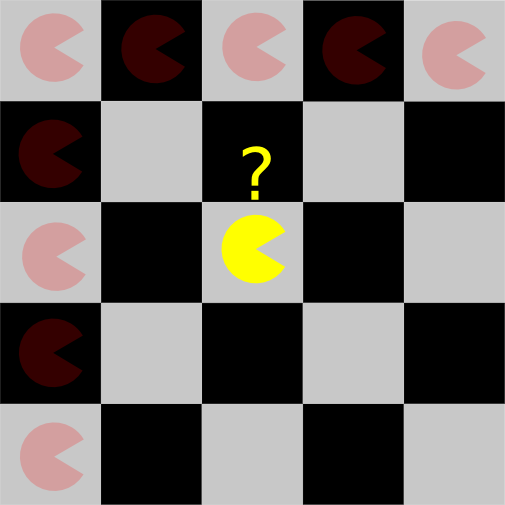
\includegraphics{Agent003.png}
    \end{column}
    \begin{column}{.48\textwidth}
      \begin{itemize}
      \item Expert's trace
      \item $MDP\backslash R $
      \item $\pi^*(s) \in \arg\max_{a\in A}Q^*(s,a)$
      \end{itemize}
      
    \end{column}
  \end{columns}
}
{.48}{3. Assumptions and Goal}{
  \begin{itemize}
  \item Assumptions
    \begin{itemize}
    \item The expert is a RL agent
    \item One can access the expert's trace
    \item The agent has the same abilities as the expert
    \end{itemize}
  \item Goal : Infer the expert's reward
    \begin{itemize}
    \item apprenticeship of the expert's task
    \item Generalization of the policy over never-seen-before states
    \item Useful when rewards are hard to tune ({\it e.g.}, driving)
    \end{itemize}
  \end{itemize}
}
{15cm}
\vfill
%%%%%%%%%%%%%%%%%%%%%%%%%%%%%%%% TROISIEME, quatrième, cinquième et sixième LIGNES
\begin{columns}
  \begin{column}{.48\textwidth}
    \begin{block}{4. Expert}
      \begin{columns}
        \begin{column}{0.001\textwidth}
          \vspace{8cm}
        \end{column}
        \begin{column}{\textwidth}
      $\pi_E(s) = \arg\max\limits_{a\in\mathcal{A}} Q^{\pi_E}(s,a)$ \hspace{12em} $\pi^C(s) \in \arg\max\limits_{a\in\mathcal{A}}q(s,a)$
          

\begin{align*}
\quality{\expertpolicy}{\expertreward}(\state,\actionBis) &= \expertreward(\state,\actionBis) + \discount \sum_{\state'\in \statespace}\transprobfunceval{\state}{\actionBis}{\state'} \quality{\expertpolicy}{\expertreward}(\state',\expertpolicy(\state'))\\
\expertreward(\state,\actionBis) &= \quality{\expertpolicy}{\expertreward}(\state,\actionBis) - \discount \sum_{\state'\in \statespace}\transprobfunceval{\state}{\actionBis}{\state'} \quality{\expertpolicy}{\expertreward}(\state',\expertpolicy(\state'))\\
\Rc(\state,\actionBis) &= \classifscorefunc(\state,\actionBis) - \discount \sum_{\state'\in \statespace}\transprobfunceval{\state}{\actionBis}{\state'} \classifscorefunc(\state',\classifpolicy(\state'))
\end{align*}

\vspace{1em}
$\classifpolicy$ is optimal for $\Rc$ and $\classifpolicy \approx \expertpolicy$, ergo we would be happy to find $\Rc$.
\vspace{1em}

$\sastrace{\sim} = \{\state_{\datasetindex},\actionBis_{\datasetindex},\state'_{\datasetindex}\}_{0\leq\datasetindex\leq\nbsamples}$\hspace{12em}
$\rsample_{\datasetindex} = q(s_{\datasetindex},a_{\datasetindex}) - \gamma q(s'_{\datasetindex},\classifpolicy(s'_{\datasetindex}))$ 
        \end{column}
      \end{columns}
    \end{block}
    \vspace{1cm}
    \begin{block}{6. Heuristics}
      \begin{columns}
        \begin{column}{0.001\textwidth}
          \vspace{8cm}
        \end{column}
        \begin{column}{\textwidth}
          $\sastrace{\expertpolicy} = \{(s_i,a_i,s'_i)_{1\leq i \leq N}\}$ \hspace{5em} $\left(s_{\datasetindex},\forall \actionBis \neq\expertpolicy(\state_{\datasetindex})\right) ,\rsample_{min} = \min_{\datasetindex\in \llbracket 1;\nbsamples\rrbracket}\rsample_{\datasetindex} - 1$
        \end{column}
      \end{columns}             
    \end{block}
    \vspace{1cm}
    %% \begin{block}{Putting it all together}
    %%   \begin{equation*}
    %%     \mathcal{X} \equiv S, \mathcal{Y} \equiv A, s\equiv Q^{\pi_E} \Rightarrow \phi \equiv \mu^{\pi_E}
    %%   \end{equation*}
    %% \end{block}
    \vfill
    \begin{block}{7. Pseudo-code}
      \resizebox{.95\columnwidth}{!}{

        \begin{algorithm}[H]
    %\small
  \caption{CSI algorithm}
  \label{algo:cascading}
  \emph{\textbf{Given}} a training set $\satrace{\expertpolicy}=\{(s_i,a_i=\pi_E(s_i))\}_{1\leq i \leq \nbsamples}$\\and another training set $\sastrace{\sim}=\{(s_{j},a_{j},s'_{j})\}_{1\leq j \leq \nbsamples'}$\;
  \emph{\textbf{Train}} a score function-based classifier on $\satrace{\expertpolicy}$, obtaining decision rule $\pi^C$ and score function $q:\statespace\times \actionspace \rightarrow \mathbb R$\;
  \emph{\textbf{Learn}} a reward function $\hat R^C$ from the dataset $\{((s_{j},a_{j}),\hat{r}_j)\}_{1\leq j \leq \nbsamples'}$, $\forall (s_j,a_j,s'_j) \in \sastrace{\sim},\hat{r}_j=q(s_{j},a_{j})-\gamma q(s'_{j},\pi_C(s'_{j}))$\;
  \emph{\textbf{Output}} the reward function $\hat R^{C}$ \;
\end{algorithm}
      }
    \end{block}
  \end{column}
  \begin{column}{.48\textwidth}
    \vfill
    \begin{block}{8. Error bound}
      With concentration coefficient $\ccoeffpi{\optimalpolicy{\apprRc}}$, classification error $\epsilon_C$ and regression error $\epsilon_R$ :
\begin{equation}
0\leq\expectationknowing{\rlvalue{\optimalpolicy{\apprRc}}{\apprRc}(s)-\rlvalue{\expertpolicy}{\apprRc}(s)}{s\sim\expertdistrib}\leq \frac{1}{1-\gamma}\left(\epsilon_C\Delta q +\epsilon_R(1+\ccoeffpi{\optimalpolicy{\apprRc}})\right).
\end{equation}
    \end{block}
    \vfill
    \begin{block}{9. Highway}
      \begin{columns}
        \begin{column}{0.001\textwidth}
          \vspace{7cm}
        \end{column}
        \begin{column}{\textwidth}
          \centering
          \fontsize{11pt}{11pt}\selectfont
          \resizebox{.95\columnwidth}{!}{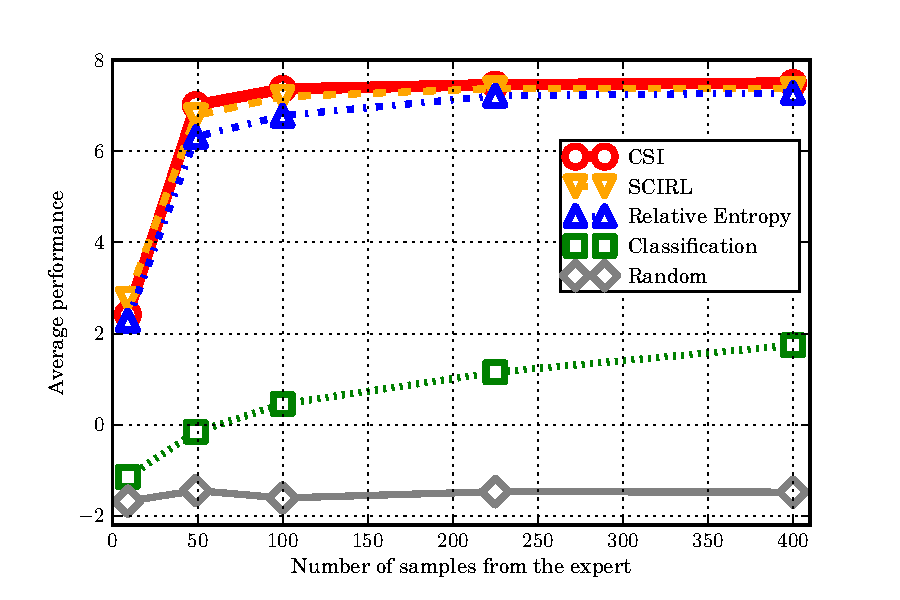
\includegraphics[width=0.47\textwidth]{Exp14}
            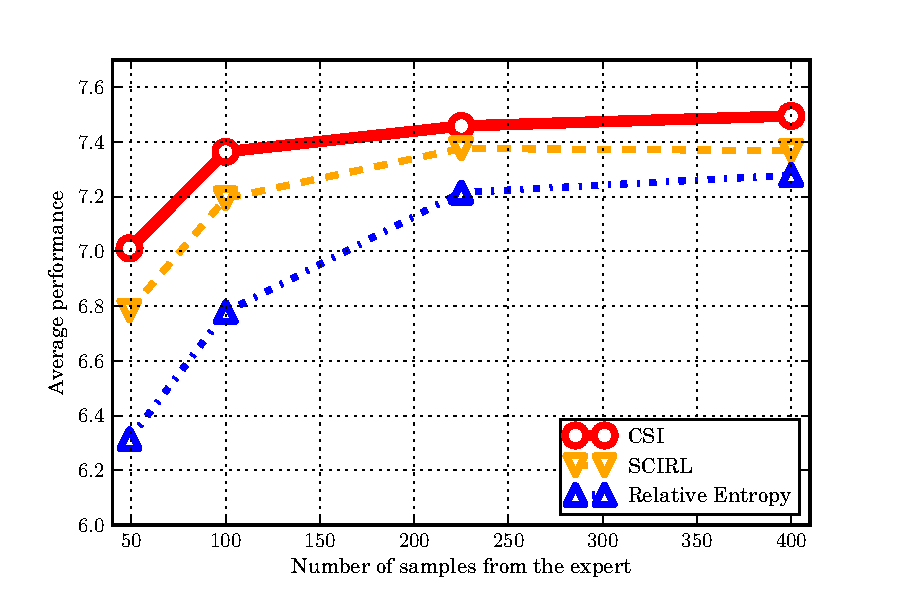
\includegraphics[width=0.47\textwidth]{Exp14_zoom}}
        \end{column}
      \end{columns}             
    \end{block}
    \begin{block}{11. Mountain Car}
      \centering
      
      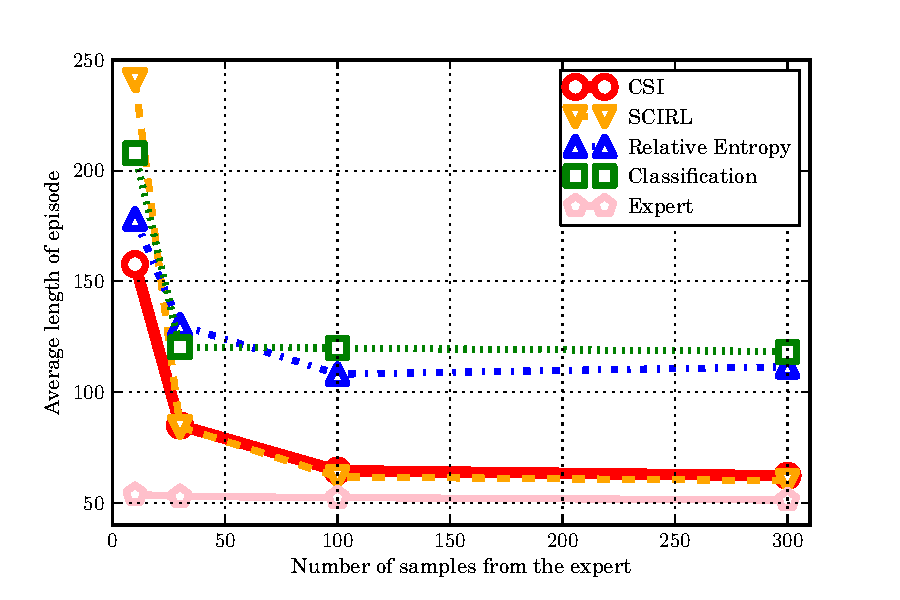
\includegraphics[width=\textwidth]{Exp11}
      %}
    \end{block}
  \end{column}
\end{columns}
\vfill



\end{frame}
\end{document}
